\chapter{Bridges, Cut Vertices, Cutsets}

Remembering that he had not told Ajur about some concepts related to connectivity of graphs and directed graphs, Rishnak went looking for Ajur and saw Ajur and Jura walking on a bridge over a small brook. Rishnak gently tapped Ajur and said that 
he wanted to talk about connectivityy. Ajur replied saying he remembered the definition of being connected - which means that there is a path between every pair of vertices. Rishnak smiled and said that it is correct.

A bridge is an edge in a connected graph that when that edge is deleted from that graph, it becomes disconnected. For the graph shown in Figure \ref{14g1}, every edge is bridge.
\begin{figure}
\begin{center}

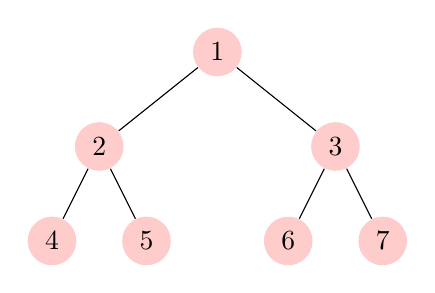
\begin{tikzpicture}
  [scale=.6,auto=left,every node/.style={circle,fill=red!20}]
  \node (n1) at (5.5,7) {1};
  \node (n2) at (3,5)  {2};
  \node (n3) at (8,5)  {3};
  \node (n4) at (2,3) {4};
  \node (n5) at (4,3)  {5};
  \node (n6) at (7,3)  {6};
  \node (n7) at (9,3)  {7};

  \foreach \from/\to in {n1/n2,n1/n3,n2/n4,n2/n5,n3/n6,n3/n7}
    \draw (\from) -- (\to);

\end{tikzpicture}
\caption{ Every edge in this graph is a bridge. In a tree, every edge is bridge!}\label{14g1}
\end{center}
\end{figure}

In the graph shown in Figure \ref{14g2}, just one edge is a bridge.

\begin{figure}
\begin{center}
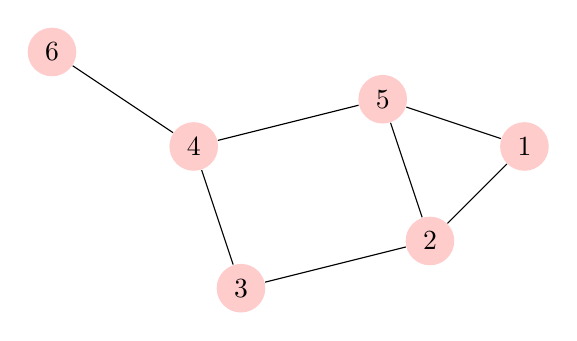
\begin{tikzpicture}
  [scale=.6,auto=left,every node/.style={circle,fill=red!20}]
  \node (n6) at (1,10) {6};
  \node (n4) at (4,8)  {4};
  \node (n5) at (8,9)  {5};
  \node (n1) at (11,8) {1};
  \node (n2) at (9,6)  {2};
  \node (n3) at (5,5)  {3};

  \foreach \from/\to in {n6/n4,n4/n5,n5/n1,n1/n2,n2/n5,n2/n3,n3/n4}
    \draw (\from) -- (\to);

\end{tikzpicture}
\caption{Edge (4,6) is the bridge}\label{14g2}
\end{center}
\end{figure}

Bridge is an important edge in a graph. If the bridge is deleted (if it fails), the graph becomes disconnected. A graph may not contain any bridge. For example, in a complete graph  there are no
bridges. If there are no bridges, there is less chance that a graph becomes disconnected when an edge is deleted.

Ajur asked Rishnak whether there is a vertex analog of a bridge. Rishnak answered in the affirmative. A cut-vertex is a vertex which when deleted \footnote{deleting a vertex means removing that vertex and removing all edges incident on that vertex.} makes the graph disconnected. In the graph shown in \ref{14g2}, vertex 4 is a cut vertex. If you consider the map of continental United States (with states as vertices and there is an edge between two vertices (states), if they share a common border), New Hampshire is a cut-vertex, if you delete New Hampshire, it is not possible to go from Maine to other states through United States. Similarly in India, West Bengal is  a cut vertex, as from north eastern state (like Assam), you cannot go to Kerala!

In a tree, all vertices other than leaf vertices are cut vertices. In a complete graph, there are no cut vertices. If a graph or a network has a cut vertex, that network is vulnerable and may get disconnected if the cut vertex fails. 

A graph is $k$ connected if there is a set of $k$ vertices which when deleted from the graph becomes disconnected. Ajur realized that $k$ connected is a generalization of 1 connected (correspond to having a cut vertex.)

A cutset is a set of edges which when deleted will make the graph disconnected. Rishnak asked Ajur how many vertices need to be deleted for the graph shown in Figure \ref{14g3} and what is a cutset for this graph.

\begin{figure}
\begin{center}

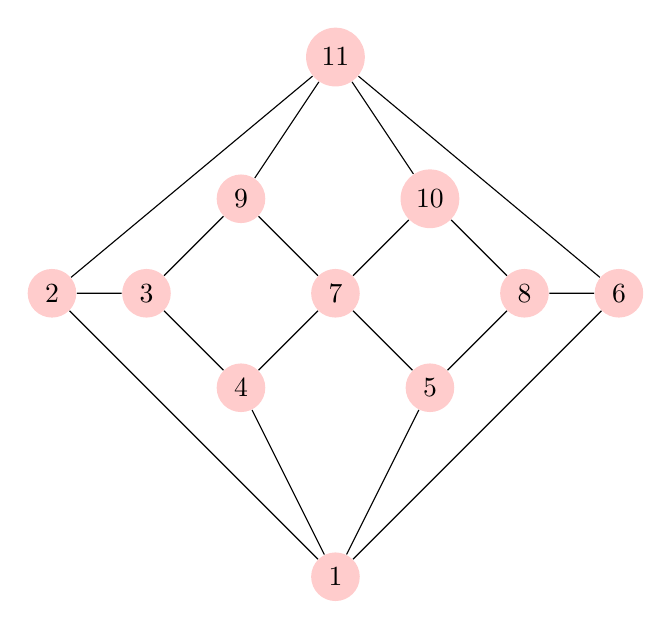
\begin{tikzpicture}
  [scale=.6,auto=left,every node/.style={circle,fill=red!20}]
  \node (n1) at (6,-3) {1};
  \node (n2) at (0,3)  {2};
  \node (n3) at (2,3)  {3};
  \node (n4) at (4,1) {4};
  \node (n5) at (8,1)  {5};
  \node (n6) at (12,3)  {6};
  \node (n7) at (6,3)  {7};
 \node (n8) at (10,3) {8};
  \node (n9) at (4,5)  {9};
  \node (n10) at (8,5)  {10};
  \node (n11) at (6,8)  {11}; 

  \foreach \from/\to in {n1/n2,n1/n4,n1/n5,n1/n6,n2/n3,n2/n11,n3/n4,n3/n9,n4/n7,n5/n7,n5/n8,n6/n8,n6/n11,n7/n9,n7/n10,n8/n10,n9/n11,n10/n11}
    \draw (\from) -- (\to);

\end{tikzpicture}
\caption{How many vertices should be deleted to make this graph disconnected? How many edges should be deleted to make this graph disconnected? }\label{14g3}
\end{center}
\end{figure}

Ajur said in a hurry that by deleting vertices 1,3, 11, the graph in \ref{14g3} will be disconnected. He
also gave a cutset consisting of edges (2,3),(2,11) and (1,2).

\textbf{Question for twelfth day:}  What is the largest number of bridges one can have in a connected graph with $n$ vertices, Draw a graph with six vertices, having exactly two bridges.

\textbf{Answer:} Ajur said that a tree is a minimally connected graph. Since every edge is in some unique path, all the edges of the tree are bridges. Hence the maximum number of bridges in a connected graph can be $n-1$. If we have $n$ or more edges, then we will have a cycle. Hence we cannot have bridges $\ge~n$.

Ajur drew the following graph Figure \ref{14ag1} which has exactly two bridges with six vertices.

\begin{figure}
\begin{center}
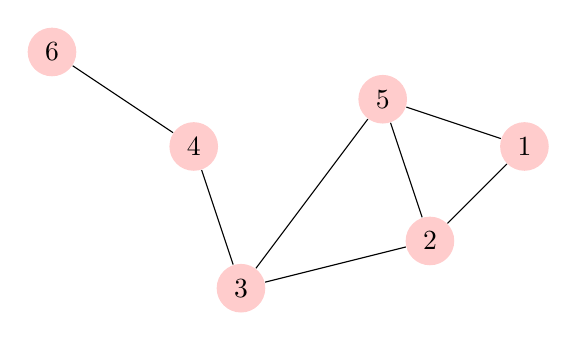
\begin{tikzpicture}
  [scale=.6,auto=left,every node/.style={circle,fill=red!20}]
  \node (n6) at (1,10) {6};
  \node (n4) at (4,8)  {4};
  \node (n5) at (8,9)  {5};
  \node (n1) at (11,8) {1};
  \node (n2) at (9,6)  {2};
  \node (n3) at (5,5)  {3};

  \foreach \from/\to in {n6/n4,n3/n5,n5/n1,n1/n2,n2/n5,n2/n3,n3/n4}
    \draw (\from) -- (\to);

\end{tikzpicture}
\caption{A graph with six vertices and two bridges (6,4) and (4,3)}\label{14ag1}
\end{center}
\end{figure}


Rishnak noticed that Ajur and Jura were getting impatient and called it a night.